\documentclass[leqno, 12pt]{article}
\usepackage{tikz}
\usetikzlibrary{positioning}
\usetikzlibrary {arrows.meta}
\usetikzlibrary{bending}
\usepackage[a4paper, portrait, margin=1cm]{geometry}
\usepackage{fancyhdr}

\def\jumpheight{10}
\def\qgap{\rule[-1pt]{1.0em}{.25pt}}

\def \HeadingQuestions {\section*{\Large Name: \underline{\hspace{8cm}} \hfill Date: \underline{\hspace{3cm}}} \vspace{-3mm}
{Number lines: Questions} \vspace{1pt}\hrule}

% raise footer with page number; no header
\fancypagestyle{myfancypagestyle}{
  \fancyhf{} % clear all header and footer fields
  \renewcommand{\headrulewidth}{0pt} % no rule under header
  \fancyfoot[C] {\thepage} \setlength{\footskip}{14.5pt} % raise page number 6pt
}
\pagestyle{myfancypagestyle}  % apply myfancypagestyle

\begin{document}
  \HeadingQuestions
  \vspace{-1mm}
  \begin{equation}
    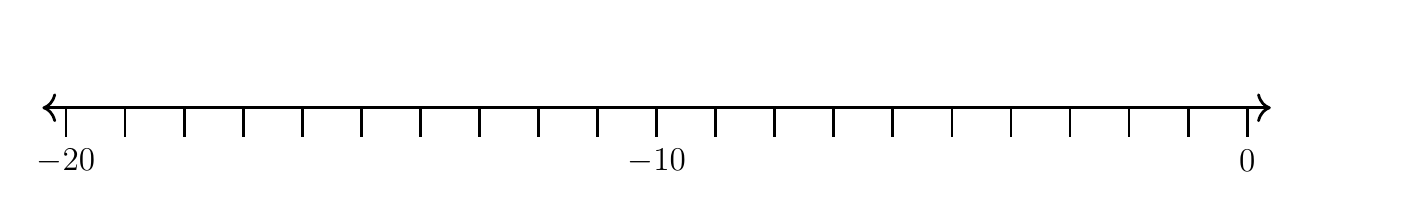
\begin{tikzpicture}[scale=0.75, baseline={([yshift=-1pt]current bounding box.north)}]
        % axis, arrow style to-to
        \draw[{To[scale=1.3]}-{To[scale=1.3]}, line width=1pt] (-20.4, 0) -- (0.4, 0);
        % tick marks
        \foreach \x in {-20,-19,...,0}
            \draw[shift={(\x,0)},color=black, line width=1pt] (0pt,-14pt) -- (0pt,0pt);
        % numbers along each axis
        \foreach \x in {-20,-10,0}
            \draw[shift={(\x,-0.8)},color=black] node[font=\large,text height=12pt] {$\x$};
        % equation at right end
        \node [font=\large, minimum width=30mm] at (0.5,1.2) {$  $};
    \end{tikzpicture}
\end{equation}

\vspace{10pt}\begin{equation}
    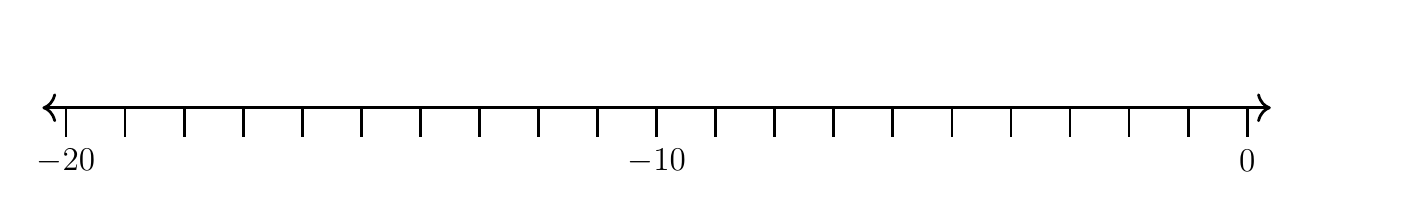
\begin{tikzpicture}[scale=0.75, baseline={([yshift=-1pt]current bounding box.north)}]
        % axis, arrow style to-to
        \draw[{To[scale=1.3]}-{To[scale=1.3]}, line width=1pt] (-20.4, 0) -- (0.4, 0);
        % tick marks
        \foreach \x in {-20,-19,...,0}
            \draw[shift={(\x,0)},color=black, line width=1pt] (0pt,-14pt) -- (0pt,0pt);
        % numbers along each axis
        \foreach \x in {-20,-10,0}
            \draw[shift={(\x,-0.8)},color=black] node[font=\large,text height=12pt] {$\x$};
        % equation at right end
        \node [font=\large, minimum width=30mm] at (0.5,1.2) {$  $};
    \end{tikzpicture}
\end{equation}

\vspace{10pt}\begin{equation}
    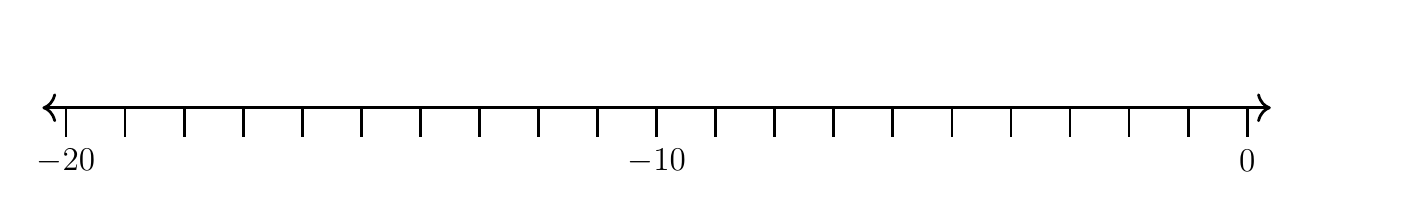
\begin{tikzpicture}[scale=0.75, baseline={([yshift=-1pt]current bounding box.north)}]
        % axis, arrow style to-to
        \draw[{To[scale=1.3]}-{To[scale=1.3]}, line width=1pt] (-20.4, 0) -- (0.4, 0);
        % tick marks
        \foreach \x in {-20,-19,...,0}
            \draw[shift={(\x,0)},color=black, line width=1pt] (0pt,-14pt) -- (0pt,0pt);
        % numbers along each axis
        \foreach \x in {-20,-10,0}
            \draw[shift={(\x,-0.8)},color=black] node[font=\large,text height=12pt] {$\x$};
        % equation at right end
        \node [font=\large, minimum width=30mm] at (0.5,1.2) {$  $};
    \end{tikzpicture}
\end{equation}

\vspace{10pt}\begin{equation}
    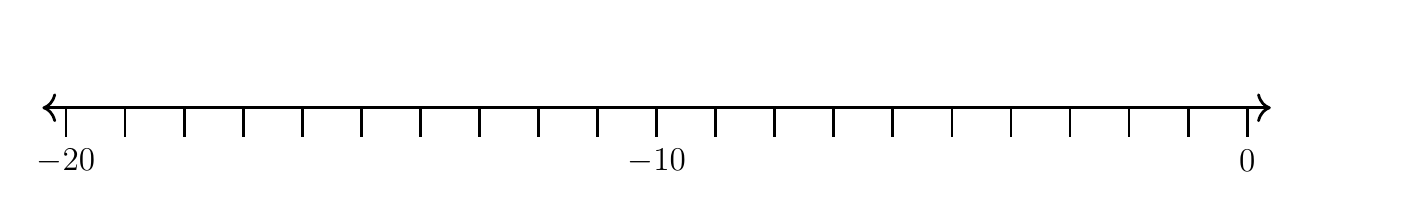
\begin{tikzpicture}[scale=0.75, baseline={([yshift=-1pt]current bounding box.north)}]
        % axis, arrow style to-to
        \draw[{To[scale=1.3]}-{To[scale=1.3]}, line width=1pt] (-20.4, 0) -- (0.4, 0);
        % tick marks
        \foreach \x in {-20,-19,...,0}
            \draw[shift={(\x,0)},color=black, line width=1pt] (0pt,-14pt) -- (0pt,0pt);
        % numbers along each axis
        \foreach \x in {-20,-10,0}
            \draw[shift={(\x,-0.8)},color=black] node[font=\large,text height=12pt] {$\x$};
        % equation at right end
        \node [font=\large, minimum width=30mm] at (0.5,1.2) {$  $};
    \end{tikzpicture}
\end{equation}

\vspace{10pt}\begin{equation}
    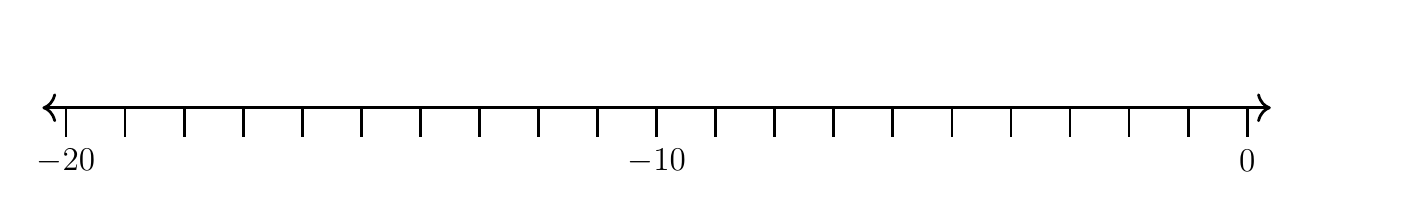
\begin{tikzpicture}[scale=0.75, baseline={([yshift=-1pt]current bounding box.north)}]
        % axis, arrow style to-to
        \draw[{To[scale=1.3]}-{To[scale=1.3]}, line width=1pt] (-20.4, 0) -- (0.4, 0);
        % tick marks
        \foreach \x in {-20,-19,...,0}
            \draw[shift={(\x,0)},color=black, line width=1pt] (0pt,-14pt) -- (0pt,0pt);
        % numbers along each axis
        \foreach \x in {-20,-10,0}
            \draw[shift={(\x,-0.8)},color=black] node[font=\large,text height=12pt] {$\x$};
        % equation at right end
        \node [font=\large, minimum width=30mm] at (0.5,1.2) {$  $};
    \end{tikzpicture}
\end{equation}

\vspace{10pt}\begin{equation}
    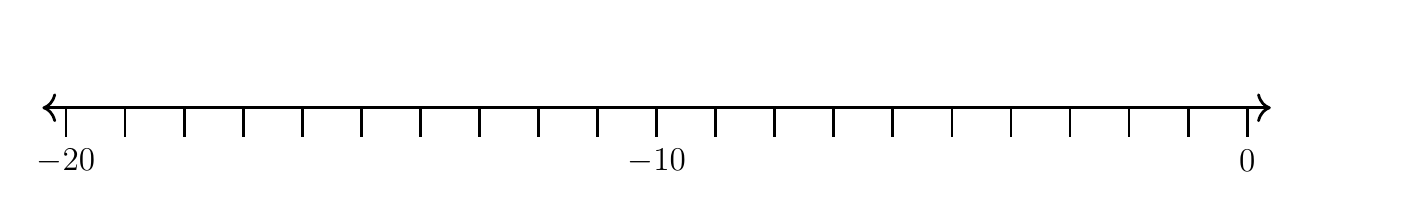
\begin{tikzpicture}[scale=0.75, baseline={([yshift=-1pt]current bounding box.north)}]
        % axis, arrow style to-to
        \draw[{To[scale=1.3]}-{To[scale=1.3]}, line width=1pt] (-20.4, 0) -- (0.4, 0);
        % tick marks
        \foreach \x in {-20,-19,...,0}
            \draw[shift={(\x,0)},color=black, line width=1pt] (0pt,-14pt) -- (0pt,0pt);
        % numbers along each axis
        \foreach \x in {-20,-10,0}
            \draw[shift={(\x,-0.8)},color=black] node[font=\large,text height=12pt] {$\x$};
        % equation at right end
        \node [font=\large, minimum width=30mm] at (0.5,1.2) {$  $};
    \end{tikzpicture}
\end{equation}

\vspace{10pt}\begin{equation}
    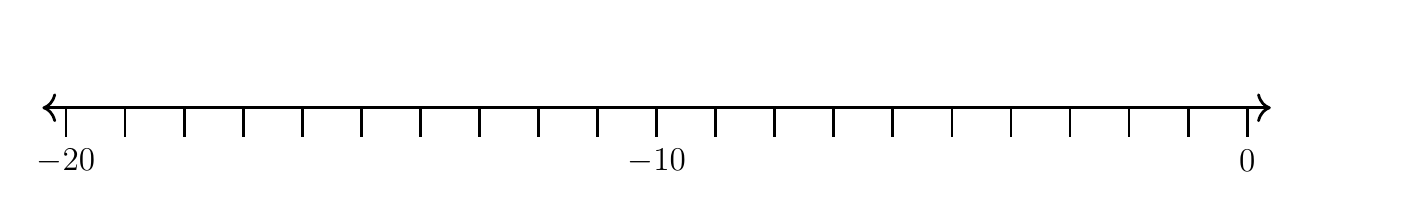
\begin{tikzpicture}[scale=0.75, baseline={([yshift=-1pt]current bounding box.north)}]
        % axis, arrow style to-to
        \draw[{To[scale=1.3]}-{To[scale=1.3]}, line width=1pt] (-20.4, 0) -- (0.4, 0);
        % tick marks
        \foreach \x in {-20,-19,...,0}
            \draw[shift={(\x,0)},color=black, line width=1pt] (0pt,-14pt) -- (0pt,0pt);
        % numbers along each axis
        \foreach \x in {-20,-10,0}
            \draw[shift={(\x,-0.8)},color=black] node[font=\large,text height=12pt] {$\x$};
        % equation at right end
        \node [font=\large, minimum width=30mm] at (0.5,1.2) {$  $};
    \end{tikzpicture}
\end{equation}

\vspace{10pt}\begin{equation}
    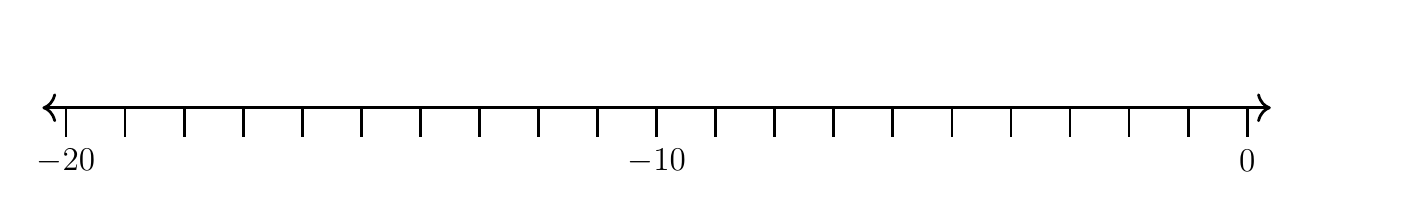
\begin{tikzpicture}[scale=0.75, baseline={([yshift=-1pt]current bounding box.north)}]
        % axis, arrow style to-to
        \draw[{To[scale=1.3]}-{To[scale=1.3]}, line width=1pt] (-20.4, 0) -- (0.4, 0);
        % tick marks
        \foreach \x in {-20,-19,...,0}
            \draw[shift={(\x,0)},color=black, line width=1pt] (0pt,-14pt) -- (0pt,0pt);
        % numbers along each axis
        \foreach \x in {-20,-10,0}
            \draw[shift={(\x,-0.8)},color=black] node[font=\large,text height=12pt] {$\x$};
        % equation at right end
        \node [font=\large, minimum width=30mm] at (0.5,1.2) {$  $};
    \end{tikzpicture}
\end{equation}

\vspace{10pt}
\end{document}

